\Titular%
{Memorias de Moscova}%
{Carlos Merino}%
{divulgacion}%
{Dpto. Física de Partículas - Facultade de Física, IGFAE\\
Universidade de Santiago de Compostela}%

\begin{refsection}
\begin{multicols}{2}

\subsection*{En homenaxe a Alexei B. Kaidalov}
%\subsection*{\small Compostela, 4 de maio de 2025}

O estudo da Física Hadrónica e da interacción forte responsable de manter aos nucleóns (protóns e neutróns) dentro do núcleo atómico e aos quarks (as partículas fundamentais que sinten esta interacción) confinados nos hadróns ten sido unha das líneas de investigación máis importantes na Física dende o fin da da Segunda Guerra Mundial e durante estas primeiras décadas do século XXI. Os avances asombrosos neste campo débense tanto ao traballo teórico máis fundamental e punteiro, como aos fitos experimentais acadados polas grandes colaboracións experimentais internacionais que en laboratorios como o Centre Européen pour la Recherche Nucléaire (CERN), de Xenebra (Suíza), desafían cada día os límites tecnolóxicos e de obtención e análise de datos. Esperamos nos conduzan a novos horizontes e retos científicos, entre eles o da obtención sistemática e completa descripción dun novo estado da materia, o plasma de quarks e gluóns (QGP), unha fase na que os quarks e gluóns están deconfinados, e que recupera o estado da materia no universo instantes despois do Big-Bang e antes da formación da materia hadrónica.

O grupo de Fenomenoloxía do Departamento de Física de Partículas e do Instituto de Física de Altas Enerxías (IGFAE) da Universidade de Santiago de Compostela leva traballando moitos anos no desenvolvemento de modelos fenomenolóxicos que permitan avanzar na predición e descrición dos datos experimentais dende a perspectiva teórica da Cromodinámica Cuántica (QCD). Esta é a teoría cuántica de campos basada no grupo de Lie non-abeliano $SU(3)$, que describe a interacción forte no Modelo Standard no que se codifica o coñecemento certo que, hoxe en día, co consenso da comunidade científica, e ratificado polo experimento, temos da realidade física e material do Universo.

En moitas ocasións, este labor de investigación das/os físicas/os do grupo de Santiago de Compostela tense levado, e segue a levarse a cabo agora mesmo, en colaboración con facultades, laboratorios e centros de investigación punteiros de moitos outros países como Alemaña, Armenia, China, Estados Unidos de América, Francia, Portugal, Ucraína, etc.

Neste senso, unha colaboración especialmente frutífera ten sido a desenvolta con grupos da antiga Unión Soviética, berce dunha das grande escolas e tradicións da Física do século XX, apoiada en algunhas das figuras máis insignes da historia da Física, como Lev Davidovich Landau, que tiveron que levar adiante o seu labor de investigación e maxisterio nunhas circunstancias vitais marcadas por uns tempos difíciles e moitas veces tráxicos.

Unha figura capital na Física Hadrónica desta escola rusa foi Alexei Borisovich Kaidalov (1940-2010), do Intituto de Física Teórica e Experimental (ITEP), de Moscova. Coñecín persoalmente a Alexei Kaidalov durante os últimos anos da década dos 80 do século pasado, durante a preparación da miña tese de doutoramento baixo a dirección de Alfóns Capella (o Profesor Carlos Pajares era codirector da tese na USC), no Laboratoire de Physique Théorique et des Hautes Énergies (LPTHE) da Université de Paris-Sud, Paris XI, en Francia, onde Alexei realizaba unha estadía de investigación para traballar con Alfóns e con Jean Tran Than Van. Lembro que, dende o primeiro momento, Alexei me causou unha grande impresión, que se viu reforzada pola paciencia e o tempo que investiu en discutir de Física co xoven estudante de doutoramento que era eu nese momento.

\begin{center}
    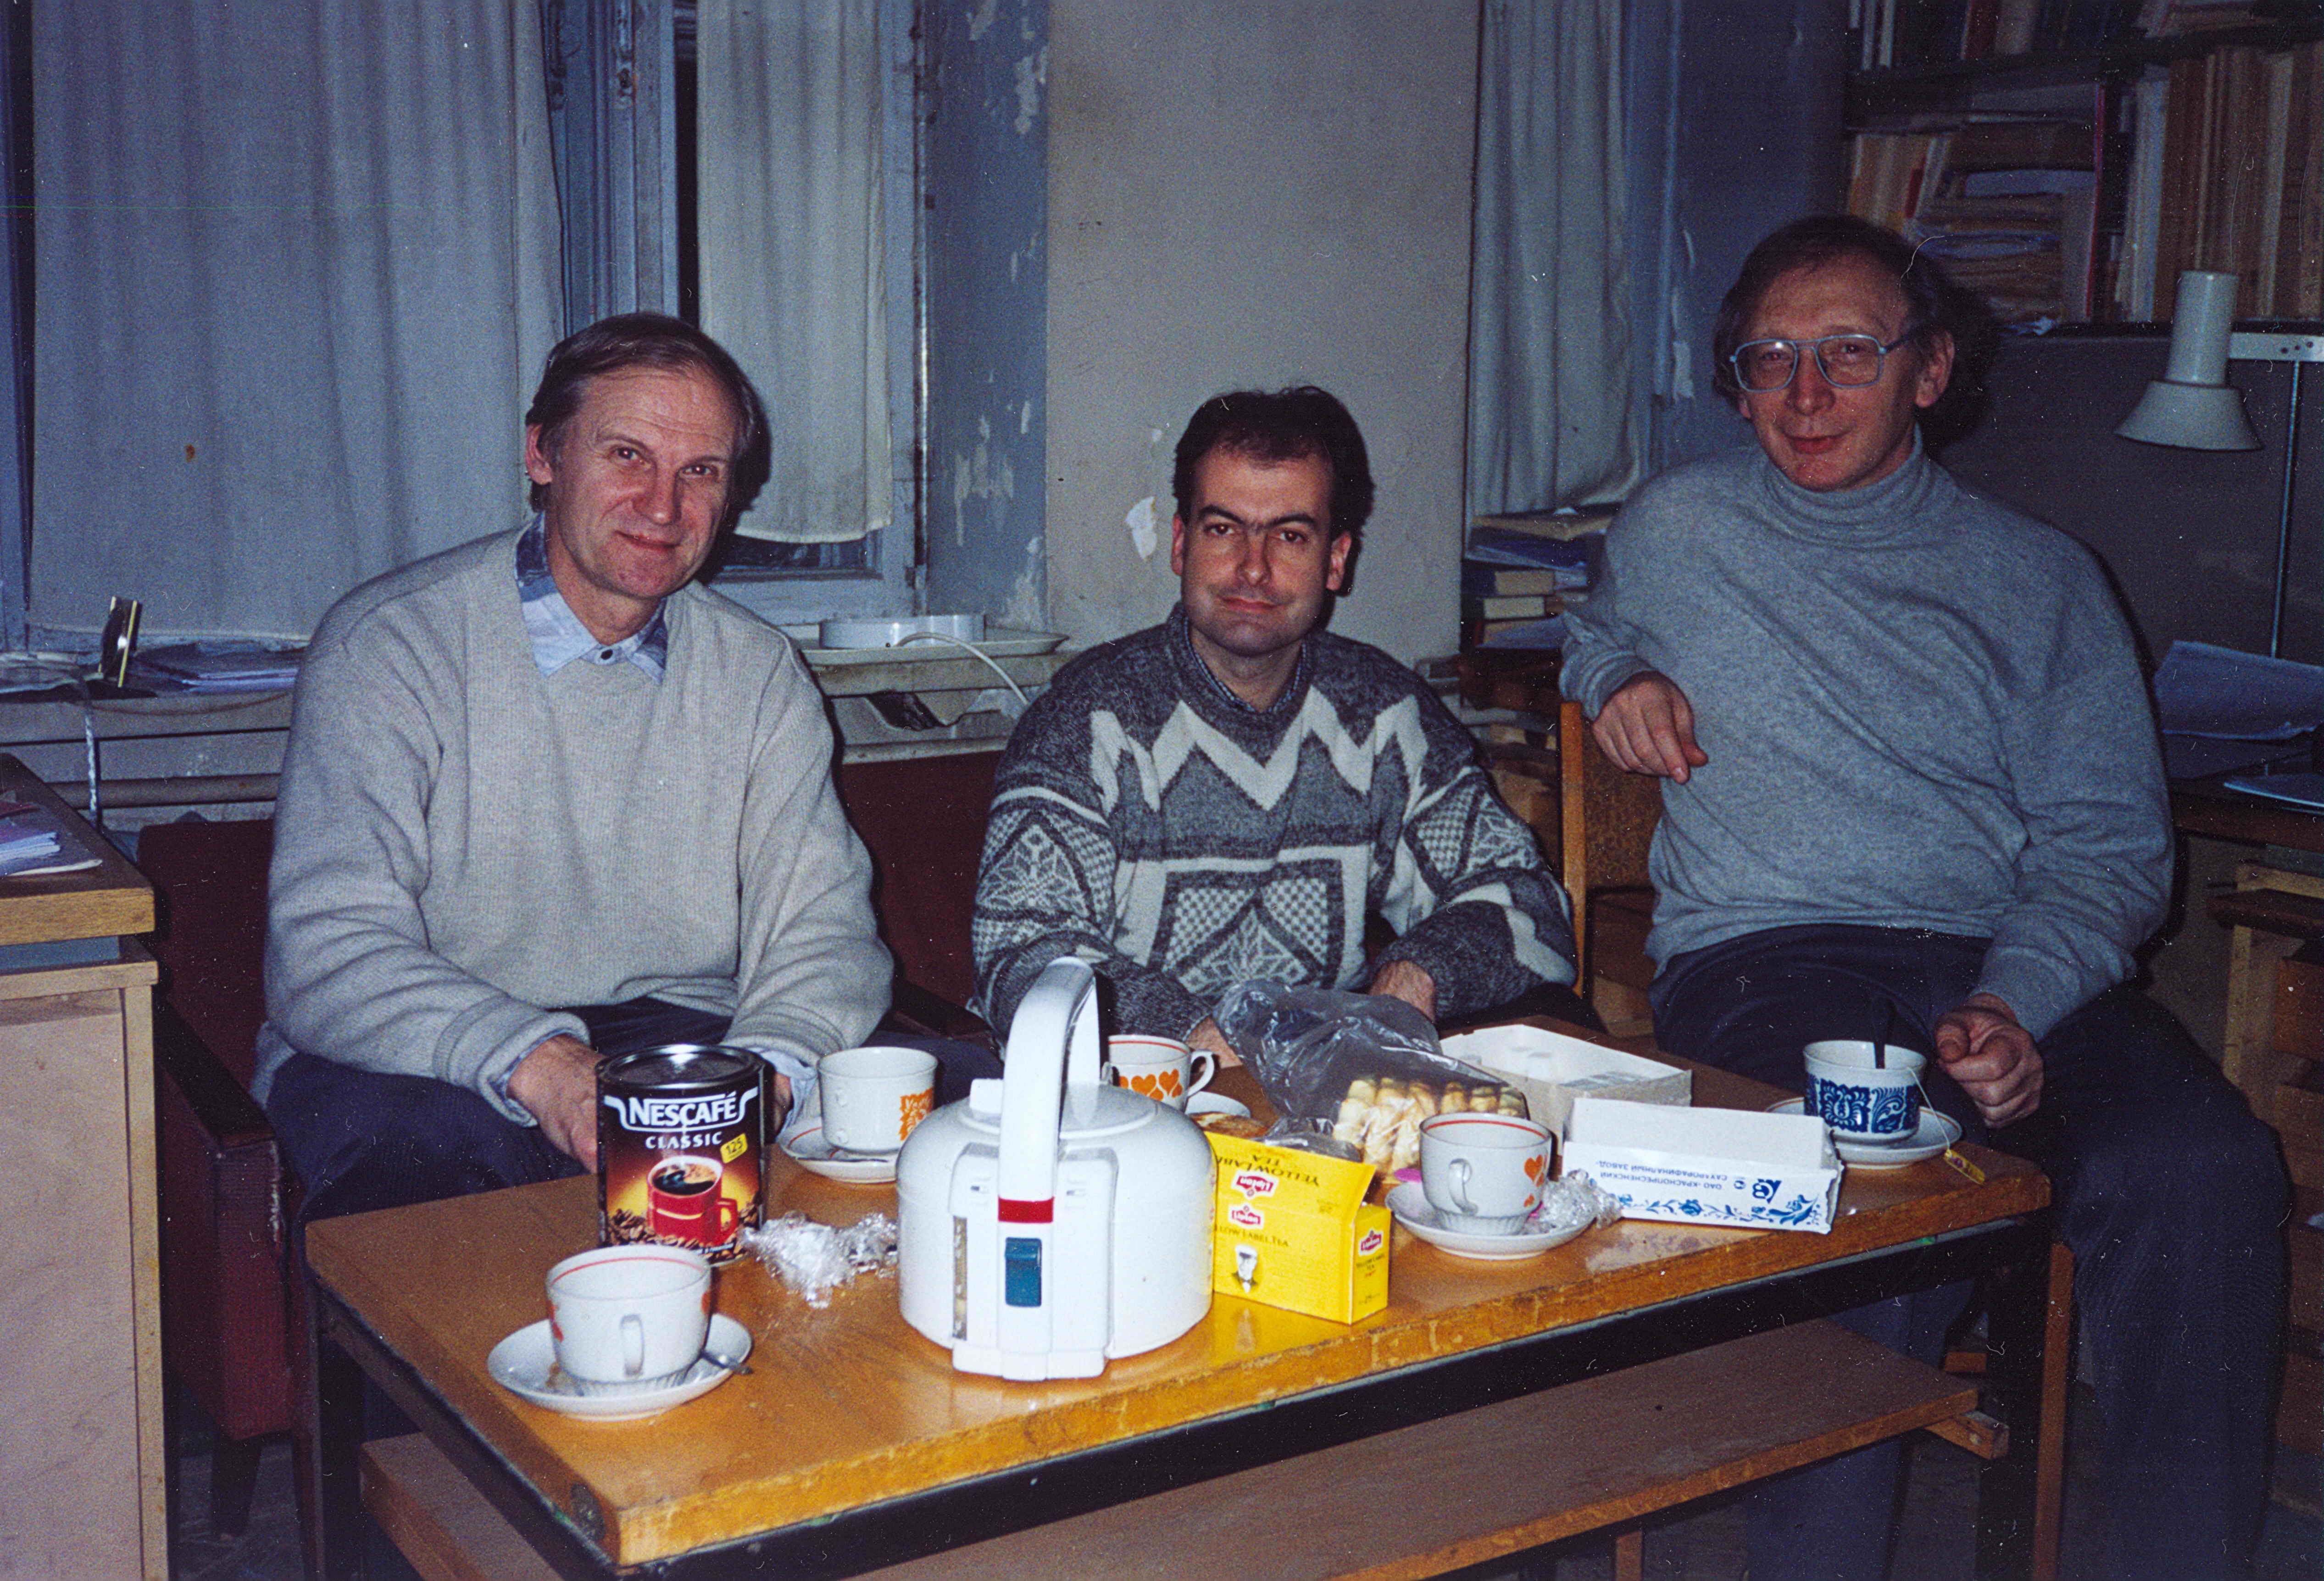
\includegraphics[width=0.9\linewidth]{revistas/002/imaxes/Kaidalov_Picture.jpg}
    \captionof{figure}{Alexei B. Kaidalov, Carlos Merino e Konstantin G. Boreskov durante unha pausa para o café/té no ITEP de Moscova (Rusia), nalgún momento en xaneiro-febreiro de 1993 (foto do arquivo de Carlos Merino).}
\end{center}    

Algún tempo despois da defensa da miña tese de doutoramento, Alexei veu a Compostela para participar, xunto con Konstantin G. Boreskov e o grande Karen A. Ter-Martirosian (alumno de Landau e mestre de Alexei, pero tamén de Gribov, Polyakov, Migdal, Zamolodchikov, e tantos outros), no XXII International Symposium on Multiparticle Dynamics, organizado polo Profesor Carlos Pajares. O feito de que físicos con tanta sona e dunha institución tan prestixiosa como o ITEP estiveran na nosa Facultade resultou moi inspirador nese momento para as/os novas/os doutoras/es que estábamos a comenzar as nosas carreiras científicas. Durante a conferencia, Alexei e Konstantin invitáronme a visitar ITEP, onde pasei un mes en xaneiro-febreiro de 1993. Ademais da extraordinaria experiencia de estar naqueles tempos nunha institución tan importante na historia da física teórica do século XX e de poder apreciar de primeira man o legado de figuras extraordinarias como Isaak Yakovlevich Pomeranchuk (do que recibe o seu nome o Pomerón, a traxectoria de Regge cos números cuánticos do baleiro que explica o aumento da sección eficaz hadrónica coa enerxía), do que Alexei foi o último alumno de doutoramento, puiden gozar dunha introdución entrañable á cultura rusa e das invitacións a compartir vodka e sakuska (os entrantes fríos que se serven como parte da comida imprescindible para acompañar a inxesta do vodka).

Vodka é o diminutivo da palabra rusa \textit{voda}, que significa auga. O vodka foi durante moito tempo un piar económico fundamental do sistema zarista, mais a finais do século XIX, a produción masiva sen ningún control, nin no procedemento nin nos ingredientes, dou lugar a unha crise de falecementos, casos de ceguera, etc. que forzara ao Zar a tomar medidas, aínda coa perda que isto podía causar ás finanzas do estado e da casa imperial. Como consecuencia desta decisión, se lle encargou a Dmitri Ivánovich Mendeléyev que atopara un método para fixar a produción regrada e evitar a proliferación de vodkas nocivos para a saúde. Mendeléyev descubriu que se se lle prendía lume a estas bebidas alcohólicas destiladas, estas ardían por enriba dos 40º de alcohol e estableceu este criterio para definir o vodka legal, que dende ese momento non pode ter unha concentración máis grande de alcohol. A partir de entón, os funcionarios do estado visitaban as granxas e as destilerías nas que se producían a bebida destilada e simplemente lle prendían lume: se a concentración de alcohol era superior aos 40º o líquido ardía e o destilador perdía o que producira. O que non ardía era o que despois a xente podía beber, pero afeitos a concentracións de alcohol moito máis grandes, ao catalo o bebedor os rusos reaccionaban decindo vodka! (auguiña!). Sexa como for, a inmensa maioría dos rusos concordan en que a Táboa Periódica foi a segunda contribución máis importante de Mendeléyev á Humanidade (a primeira, foi, sen dúbida, o vodka).

Nunha desas ocasións nas que fun invitado a unha reunión no apartamento dun dos membros do ITEP para falar, beber vodka e comer sakuska, lembro que cando chegábamos ao lugar do encontro a media tarde, despois de saír do laboratorio, Konstantin G. Boreskov máis eu facíamos os últimos metros a pé, a temperatura era moi baixa (varios graos por debaixo de cero graos celsius), e a sensación térmica era de moito frío. Despois, ao cabo de varias horas, xa de noite, arredor da medianoite, ao saírmos do edificio para coller o último metro de volta a Profsoiuznaia (Unións Profesionais-Sindicatos), a estación no suroeste do Moscova máis preta á residencia na que me aloxaba, aínda que a temperatura era moito máis baixa e o aire era glacial, tiven a impresión de non sentir tanto frío como á chegada e comenteillo a Boreskov que, cun sorriso na boca e alzando o dedo índice da man dereita cuberta pola luva, díxome: "Querido Carlos, agora xa entendes por que os rusos bebemos vodka!".

Máis tarde, a principios de 1994, cando eu estaba a realizar un postdoc no LPTHE, Alexei veu pasar uns meses no laboratorio. A súa presenza tivo un impacto inmediato na actividade investigadora do grupo dirixido por Alfóns Capella, o que se traduciu na publicación de varios papeis adicados á descripción da física de baixo-$x$ e publicados en revistas internacionais de primeiro nivel, e dos que tiven o privilexio de ser co-autor.

Nestes anos en París, que Alexei visitou máis veces e durante moitos anos despois, coincidín con Alexei en moitas conferencias e meetings, en particular en Les Reancontres de Moriond, organizados cada mes de marzo por Jean Tran Than Van nos Alpes, ben en Les Arcs ou Méribel (Francia), ben en La Thuile (Italia), e onde as fazañas no esquí de Alexei case igualaban a brillantez das súas charlas de Física. Sempre me admirou como Alexei era quen, despois de adicar as tardes a esquiar e de pasar moitas horas a discutir coas/os participantes teóricos e experimentais na conferencia que viñan pedirlle a súa opinión e o seu consello sobre os problemas máis diversos nos que estaban a traballar, de preparar unha charla final tan precisa e completa, que proporcionaba unha imaxe clara e total da actividade e dos resultados científicos presentados durante a conferencia, e das súas perspectivas de futuro. É ben coñecida a anécdota de cando no instante despois de finalizar e enviar para a súa publicación, con outros colegas, un papel moi importante que tiña requerido un esforzo moi grande, mentres os outros colegas respiraban relaxados, Alexei, sen solución de continuidade, simplemente se dirixiu ao seu escritorio, colleu (antes da existencioa dos ordeadores personais) papel e lapis e comezou a escribir, impasible, o seguinte artigo, que tiña xa redactado de principio a fin na súa cabeza.

Colaborei con Alexei durante case vinte anos, en funcións de estrutura, disociación difractiva, difracción \textit{hard}, producción de barións estraños, funcións de estrutura nuclear e demais, e somos co-autores dunha decena de papeis, pero son plenamente consciente de que esta bagaxe representa unha parte mínima do labor titánico e dos logros fundamentais que Alexei Kaidalov ten aportado á Física de Partículas. Posiblemente Alexei foi o maior experto mundial en difracción, e unha lista moi breve das súas contribución máis importantes podería ser a seguinte: \textbf{1.} A consideración das desintegracións non-leptónicas e radiactivas de hiperóns; \textbf{2.} A identificación das sinaturas dos cortes running de reggeóns nos datos experimentais; \textbf{3.} A reformulación do modelo de intercambio de un pion no marco do enfoque reggeónico e as consecuencias cuantitativas na descrición dunha grande cantidade de datos experimentais; \textbf{4.} A análise dos procesos de disociación difractiva a altas enerxías; \textbf{5.} O desenvolvemento das regras de suma para a dispersión reggeón-hadrón, que permite predecir algunhas resonancias de espín elevado; \textbf{6.} A formulación do Modelo de Cordas Quark-Gluón (QGSM) para a multiprodución a enerxías altas e moi altas, que permitiu a descrición cuantitativa dunha grande cantidade de datos experimentais en colisións hadrón-hadrón, hadrón-núcleo e núcleo-núcleo; \textbf{7.} A descrición da produción de partículas en colisións de ións pesados e dos efectos de apantallamento nuclear inelástico; \textbf{8.} A análise dos quarks pesados a da produción de pares de leptóns en colisións sobre albos nucleónicos e nucleares.

Ao longo da súa extraordinaria carreira, Alexei Kaidalov foi autor e co-autor de máis de trescentos artigos científicos publicados, dos que máis de vinte teñen cen ou máis citas, mantivo colaboracións con moitos grupos doutros países e foi membro da colaboración experimetal ALICE, do CERN. As/os profesoras/es Néstor Armesto, Elena González Ferreiro e Carlos A. Salgado, do Departamento de Física de Partículas da Facultade de Física e do IGFAE da USC, traballaron tamén con Alexei Kaidalov e son co-áutoras/es con el de artigos publicados en revistas especializadas.

Alexei Kaidalov foi un mestre respectado e admirado por colegas e amigos de todo o mundo, primeiro
polas súas moitas e moi importantes, a miúdo fundacionais, orixinais achegas ao campo da Física de Partículas, pero tamén en especial pola súa grande xenerosidade ao transmitir ás novas xeracións de físicas e físicos, a través de explicacións claras, intuitivas e rigurosas, o seu profundo coñecemento dos principios e regras que rixen os procesos físicos. Ademais da súa adicación en corpo e alma á Física, Alexei foi unha persoa optimista (maravilloso cantante do repertorio populas ruso), de mente cultivada e aberta, que valoraba moito a familia e a amizade e que estaba moi orgulloso do seu país e da súa cultura\footnote[1]{Curiosamente, cando no ano 2013, os organizadores do \textit{1st International Kaidalov Workshop on the Phenomenology of High Energy Particle Physics}, adicado á memoria de Alexei, me pediron que escribira unha semblanza [1] (en inglés) sobre el, os amigos e colegas rusos que leron o manuscrito antes da súa publicación pedíronme que non utilizara o termo cosmopolita, que nas demais linguas ten unha connotación positiva e eu empregábaa como un eloxio, porque en ruso, e dende os primeiros anos da Revolución Bolxevique, \textit{kosmopolitichnyy} ten o sentido negativo de axente estranxeiro, persoa decadente ou traidor.}.

Colaborar con Alexei Borisovich Kaidalov ten significado para min ao poder aproximarme á excelencia na Física e a apreciar un exemplo de ética no traballo e de integridade na vida, que nos debe guiar na seriedade e xenerosidade cara aos demais no noso labor académico e de investigación e que, ademais, nos debe reafirmar no convencemento da valía das/os graduadas/os na Facultade de Física da USC para, a través do traballo persoal, colaborar activamente de xeito positivo coas físicas e físicos de calquera outra universidade ou centro de investigación do mundo.

\subsection*{Agradecementos}

O autor quere felicitar aos membros da DAF polo seu traballo a prol da vida e actividade da Facultade, e ao estudantado pola iniciativa de recuperar a revista da Facultade, plataforma na que compartir experiencias e inquedanzas, alumnas/os, profesoras/es e persoal de administración e servizos, que desexo se vexa refrendada polo éxito. Agradezo a Sebastián Táboas e a todo o Comité Editorial da revista, a súa invitación a contribuír con este artigo neste segundo número e a súa paciencia á hora de ser indulxentes co prazo de entrega do mesmo, e a Belén Merino a súa revisión do texto. Espero que este segundo número de \textit{Momentum} teña continuación en moitos máis números no futuro. 

\nocite{Merino_2015}

\printbibliography

\end{multicols}
\end{refsection}